\documentclass[./main.tex]{subfiles}

\begin{document}

\chapter{ SYSTEM DESIGN}
\addtocontents{lof}{\protect\addvspace{-10pt}}
\noindent
This chapter gives an overview of the proposed system along with defining
the system architecture and UML diagrams such as use-case and class diagrams. A
UML diagram is a diagram based on the UML (Unified Modelling Language) with
the purpose of visually representing a system along with its main actors, roles,
actions, artifacts or classes, in order to better understand, alter, maintain, or document
information about the system.


\section{Overview of System Design}
\noindent
We are implementing a system that will create a predictive model using a custom training algorithm. Users can make decisions to buy or sell stocks based on the model's predictions. The system will calculate profit or loss based on the closing price of a stock for the day, which we consider as the target variable.

\noindent
Forecasting stock market behavior can seem complicated because there are many unknown factors that don't seem to follow a straightforward pattern. However, by using machine learning effectively, we can teach computers to recognize trends and make informed guesses by looking at past and current data.
\begin{figure}[H]
  \centering
  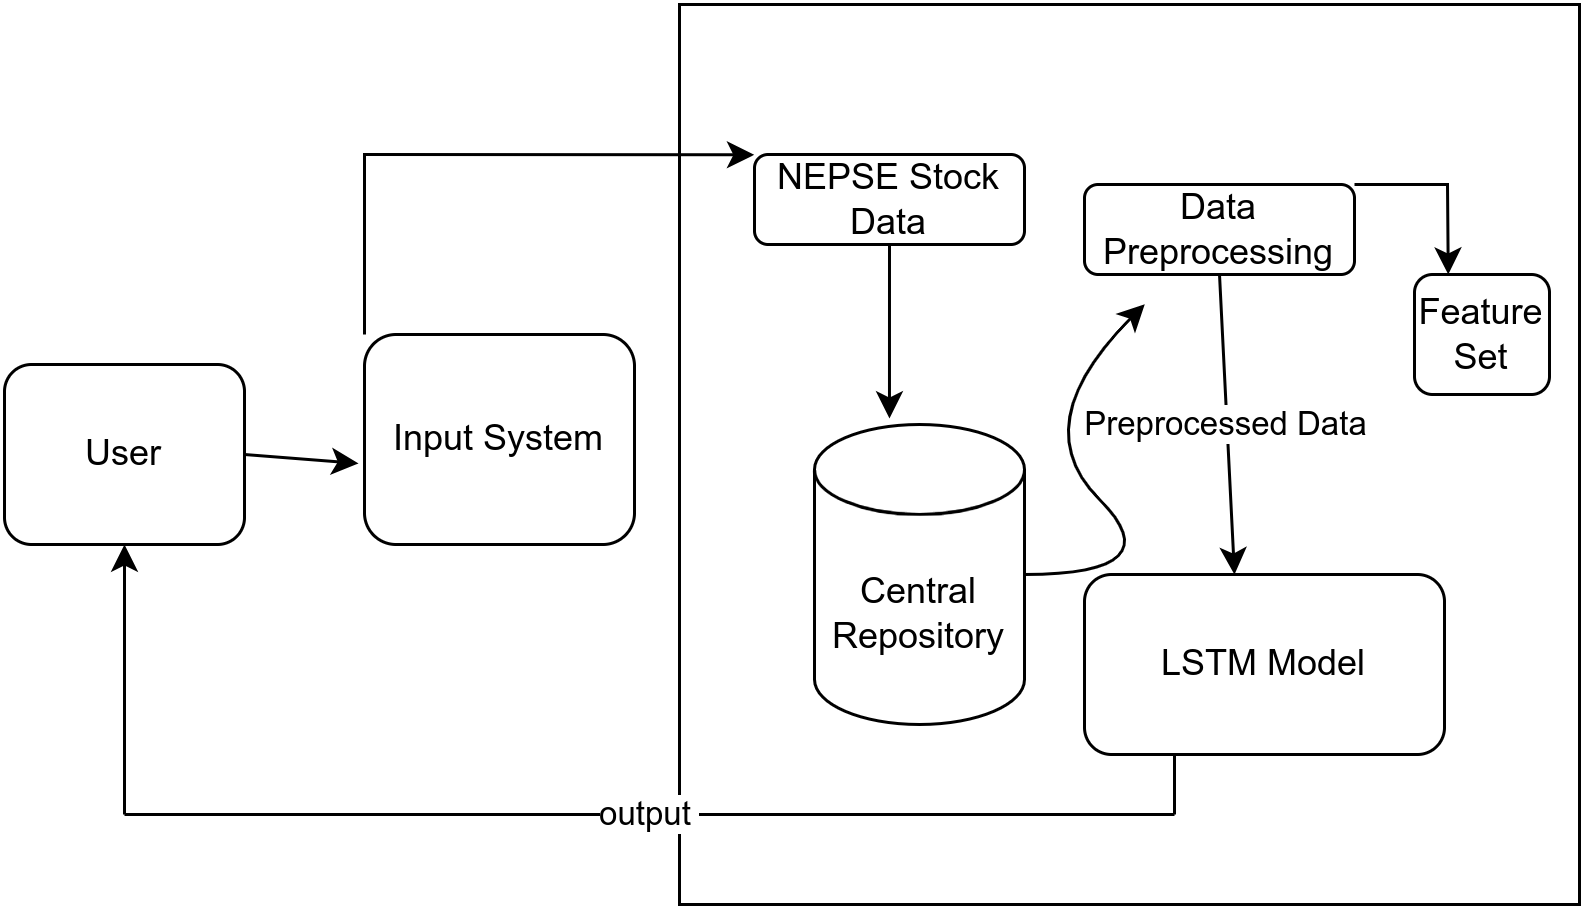
\includegraphics[width=0.50\linewidth ]{images/Architecture.png}
  \caption{System Architecture}
  \label{fig:4.1}
\end{figure}

\section{System Flow Diagram}
\begin{figure}[H]
    \centering
    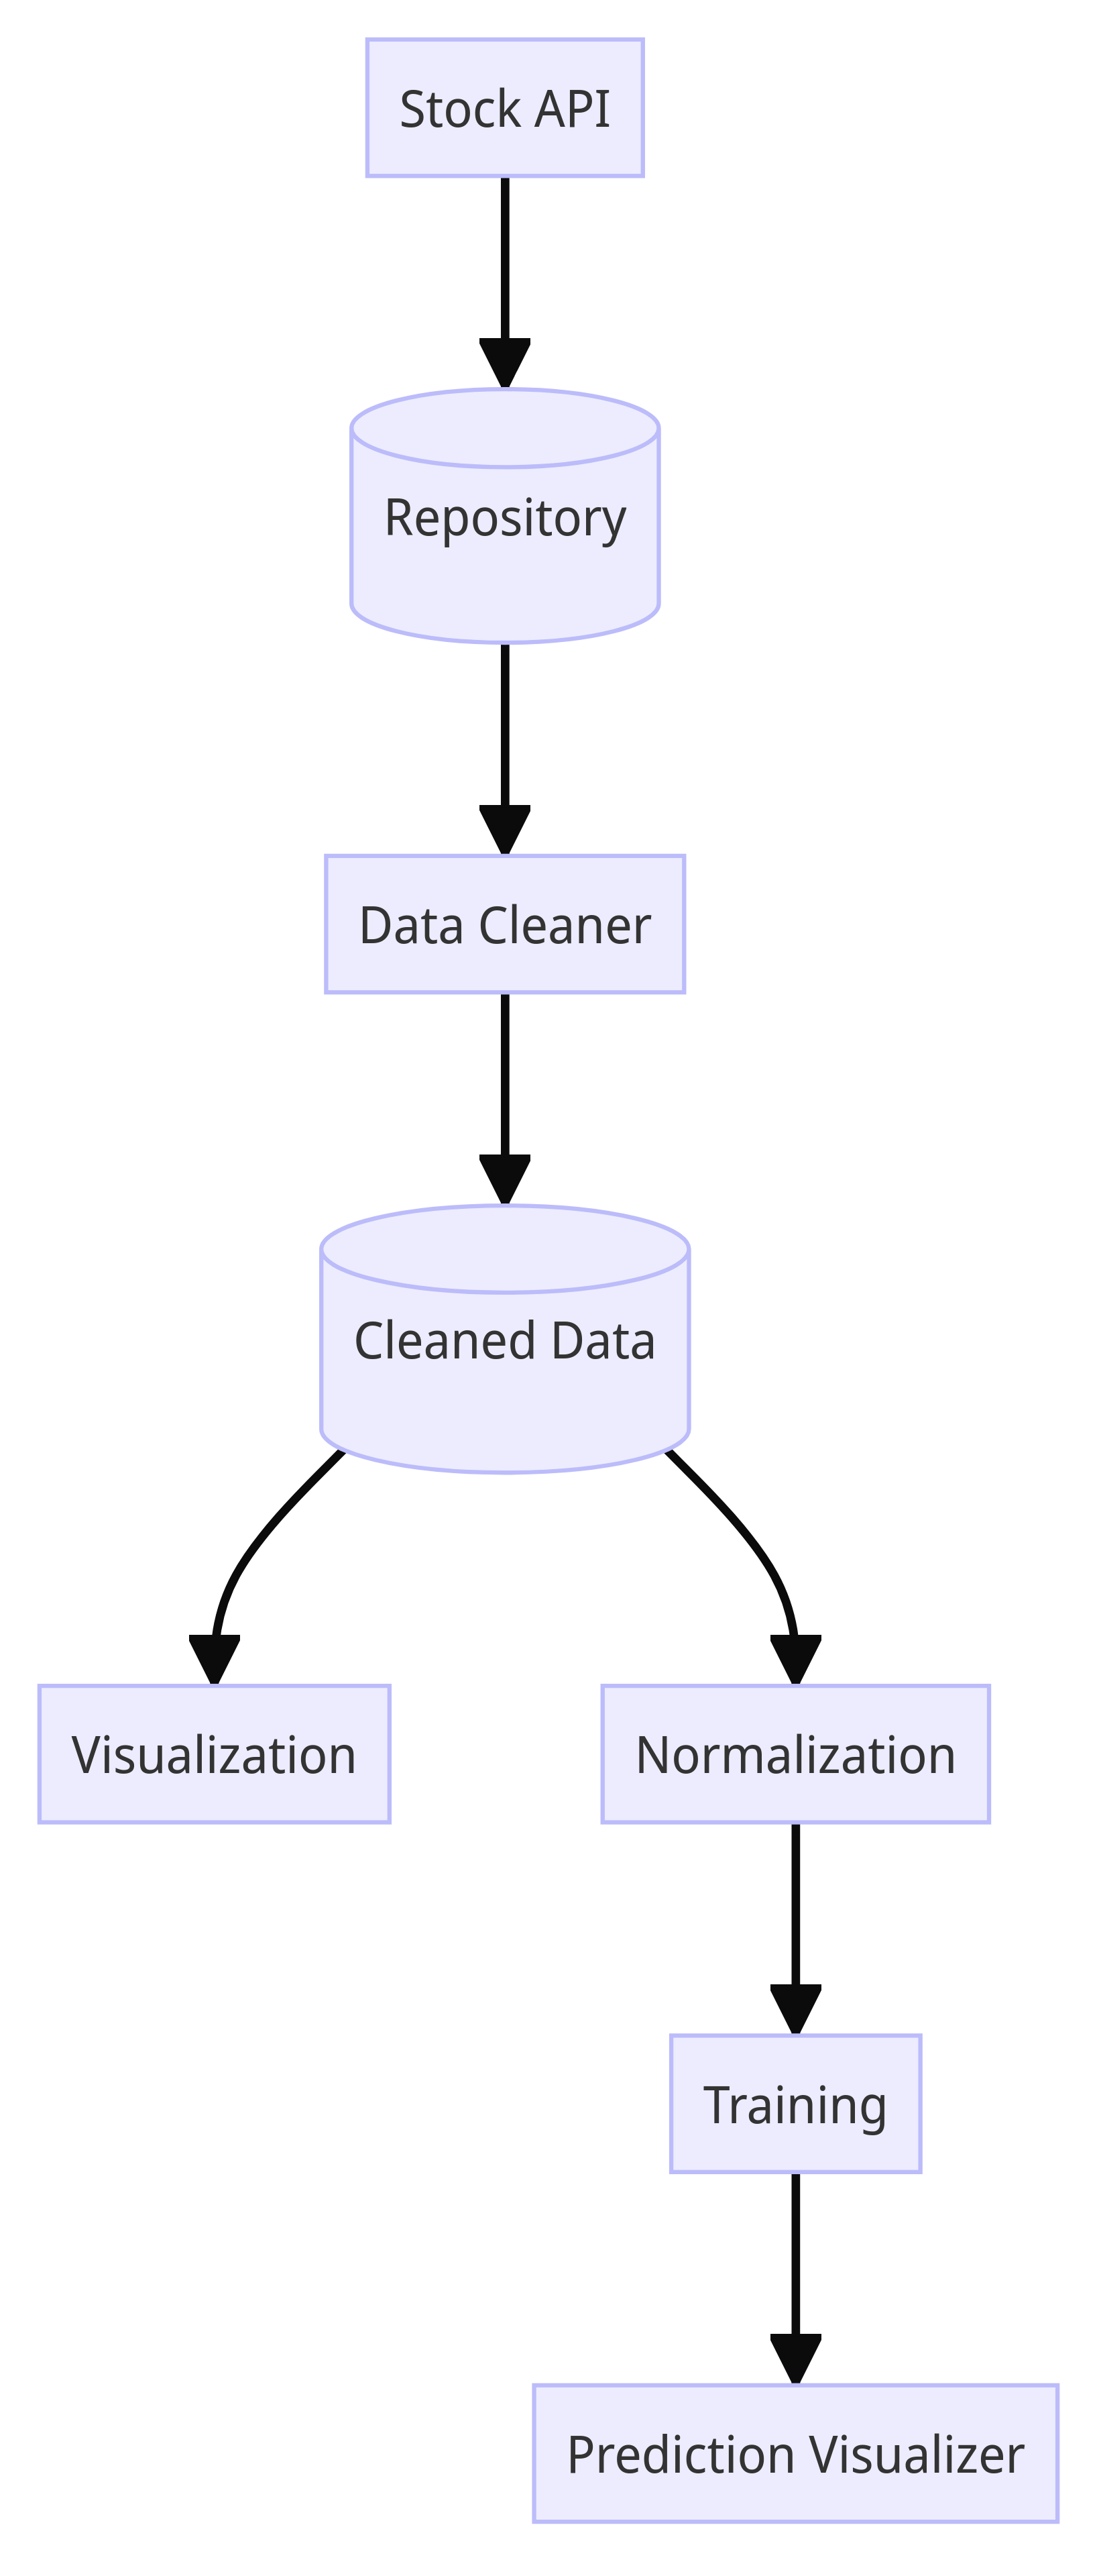
\includegraphics[width=0.50\linewidth ,height=15cm]{images/SystemDiagram.png}
    \caption{System Flow Diagram}
    \label{fig:4.2}
\end{figure}


\noindent The system flow diagram illustrates the process whereby our system retrieves data from stock APIs and stores it in a central repository. Subsequently, the data undergoes cleaning, visualization, normalization, and training stages before predictions are generated.

 \section {Activity Diagram}
 \begin{figure}[H]
     \centering
        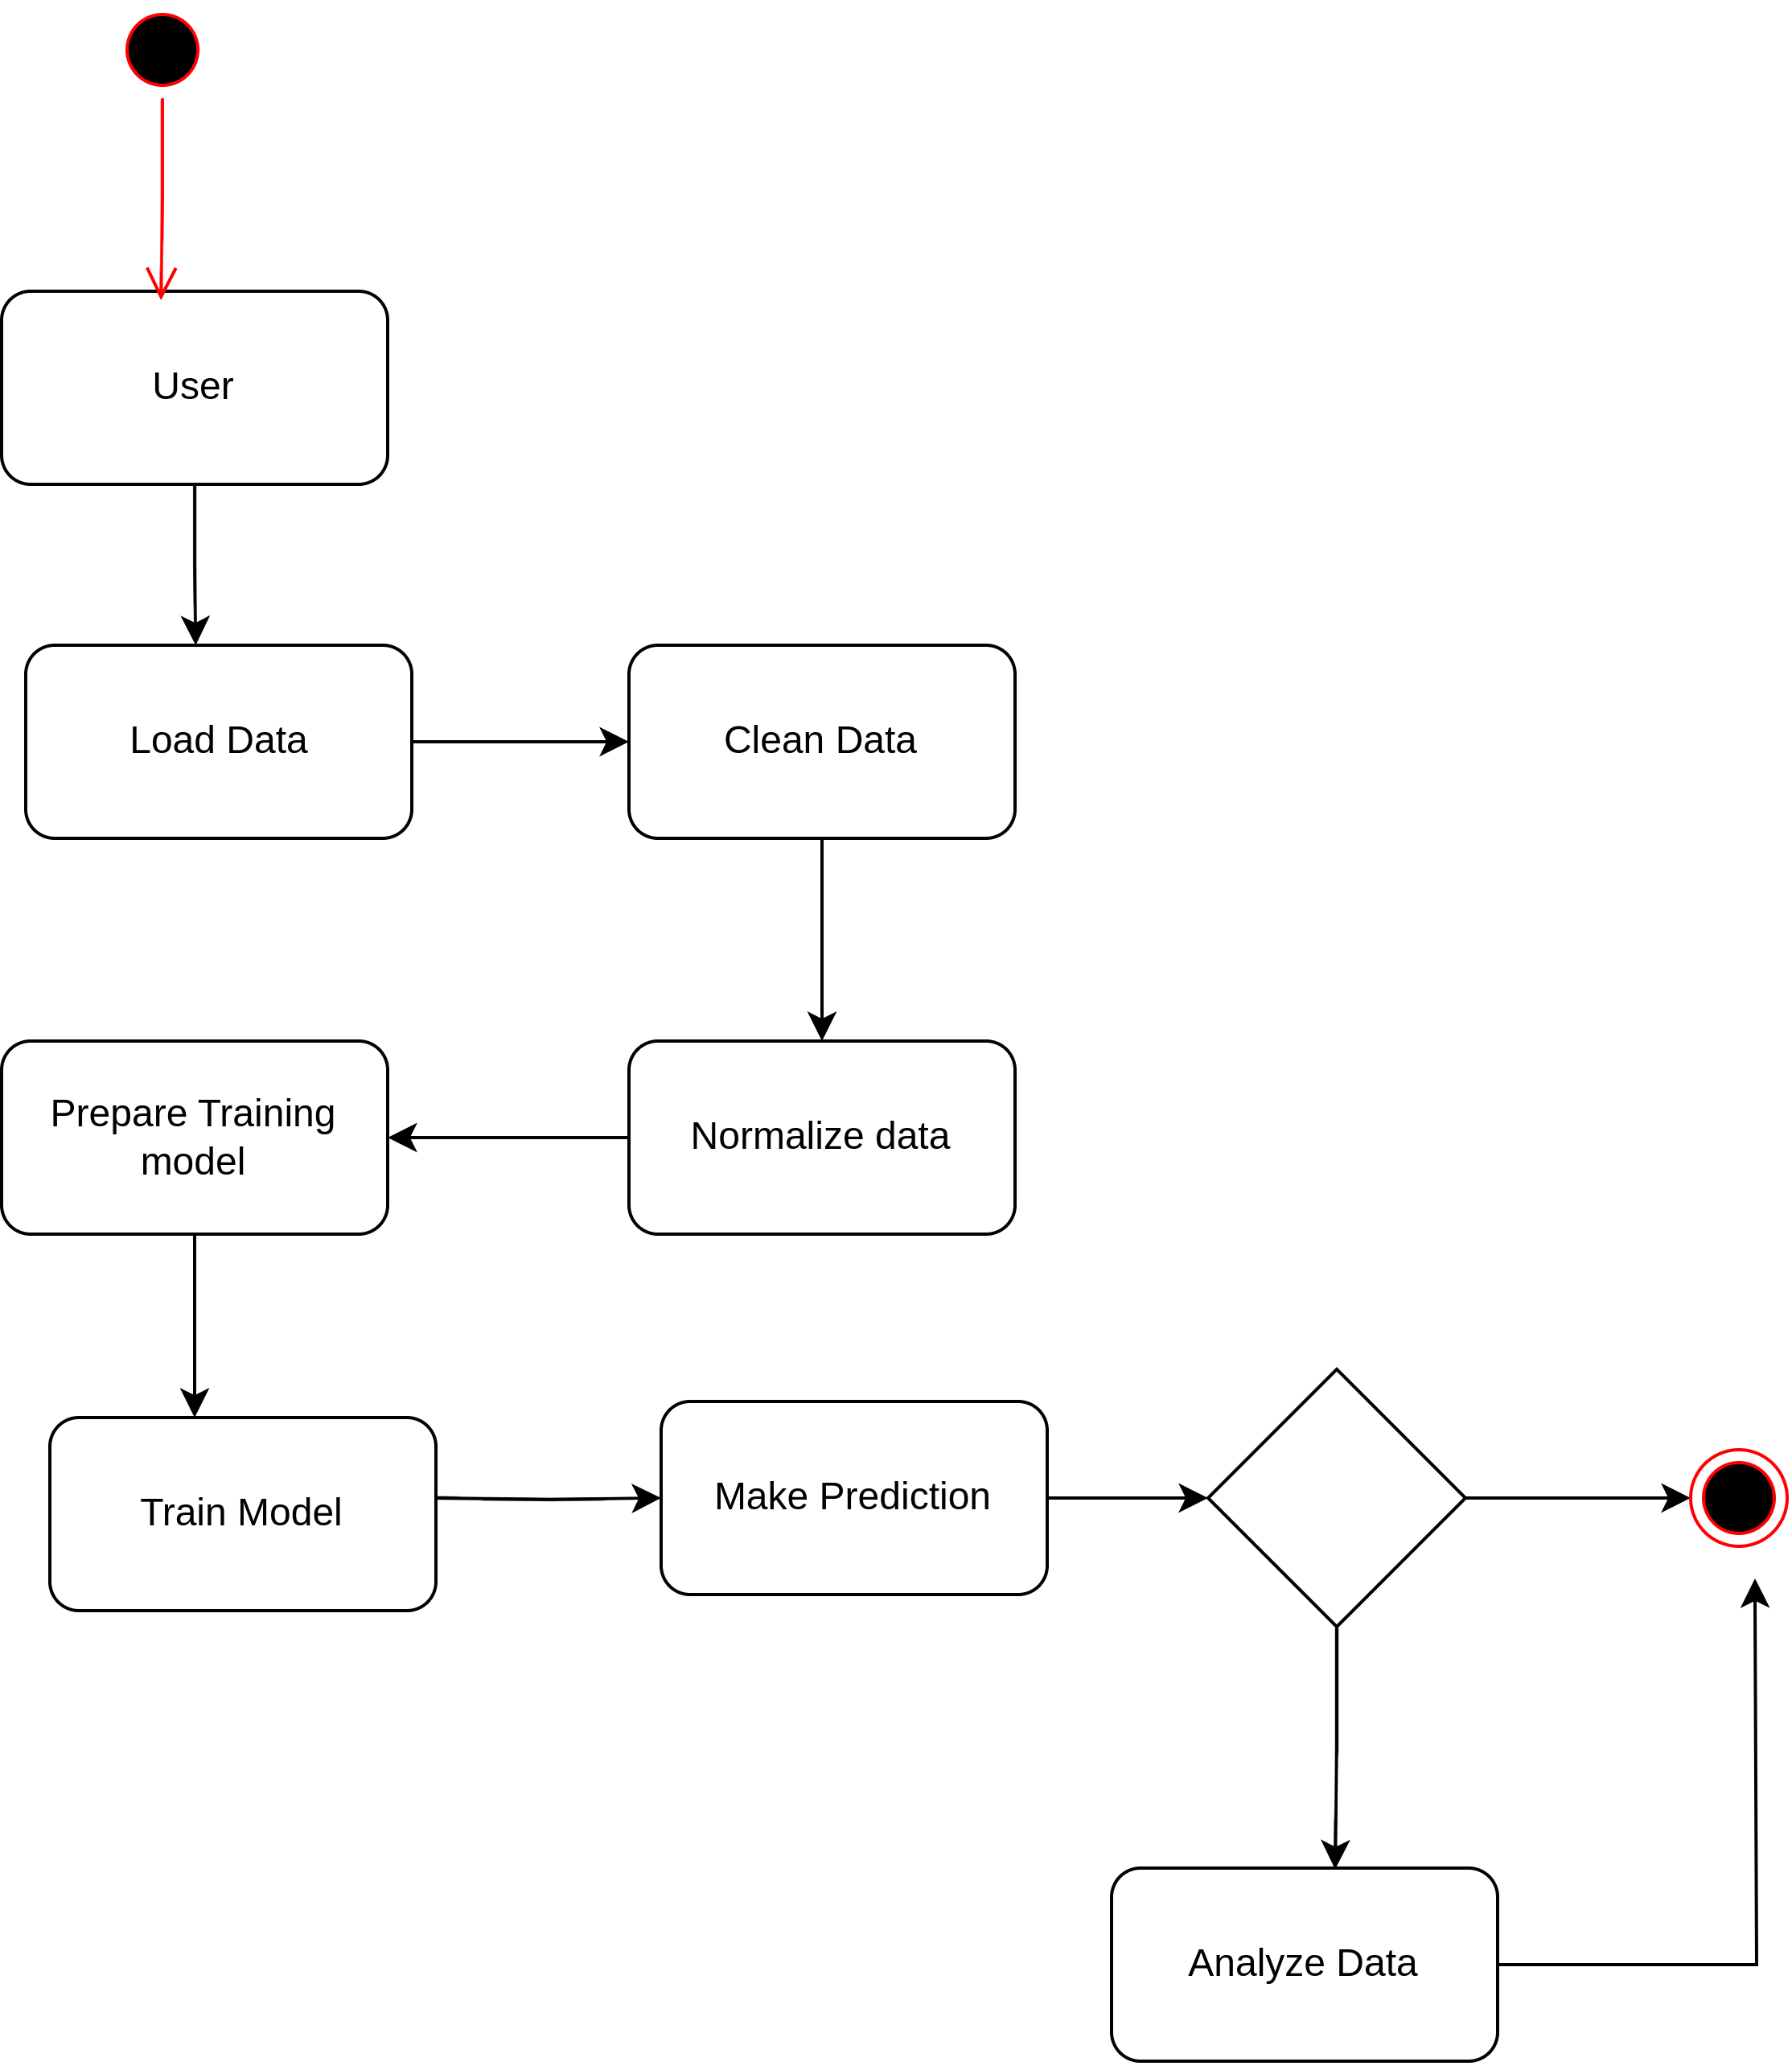
\includegraphics[width=1\linewidth,height=15cm]{images/activity.png}
     \caption{Activity Diagram}
     \label{fig:4.3}
 \end{figure}
\noindent The activity diagram fot the system shows the process of data collection, preprocessing, model training, and prediction generation. The system will also provide visualizations of the historical and predicted stock prices.
\section{Class Diagram}

\begin{figure}[H]
    \centering
    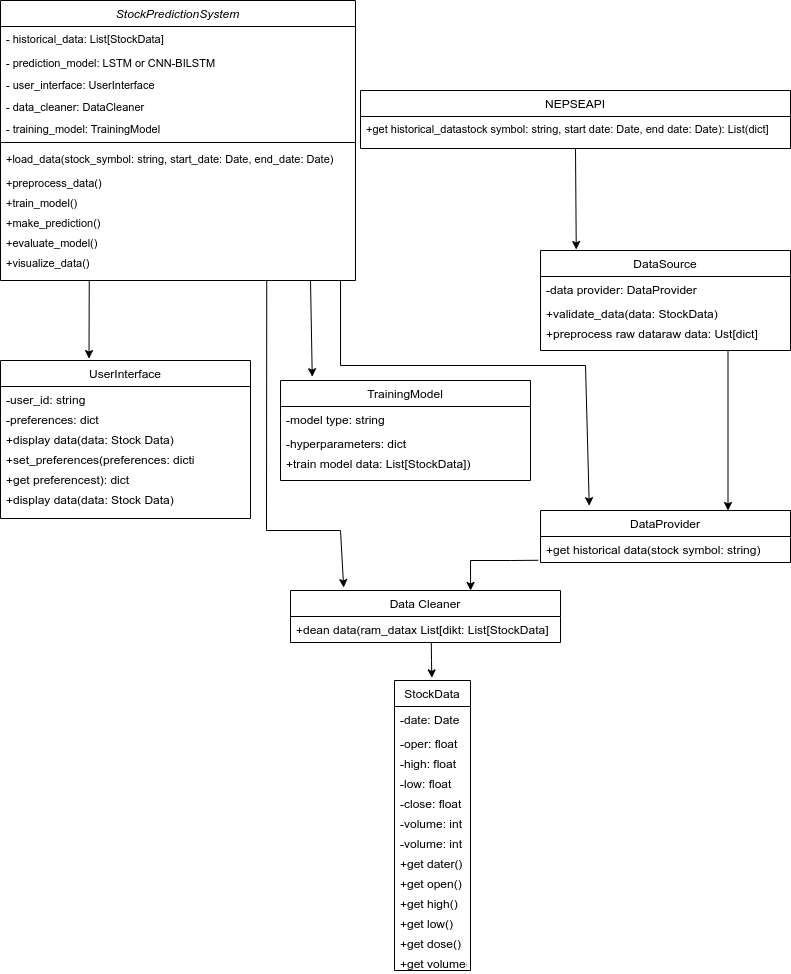
\includegraphics[width=1\linewidth]{images/ClassDiagram (1).png}
    \caption{Class Diagram}
    \label{fig:4.4}
\end{figure}
 \noindent 
The class diagram delineates the connections and data flow between base and derived classes. Within the system, the Datasource class is responsible for collecting data from the stock API and storing it centrally. The DataCleaner class performs data cleaning and normalization tasks, while the TrainingModel class handles model training and prediction generation. Serving as the foundation for the application, the StockPredictionSystem class manages user functions and interacts with the other classes.
\section{Algorithm Details}
We are using LSTM algorithm for our project. LSTM is a special kind of RNN, which shows outstanding performance on a large variety of problems. LSTM is well-suited to classify, process and predict time series given time lags of unknown duration. It trains the model by using backpropagation. Backpropagation is a method used in artificial neural networks to calculate a gradient that is needed in the calculation of the weights to be used in the network. Backpropagation is shorthand for "the backward propagation of errors," since an error is computed at the output and distributed backwards throughout the network's layers. It is commonly used to train deep neural networks, a term referring to neural networks with more than one hidden layer. \cite{intellipaat-lstm}

\begin{figure}[H]
    \centering
    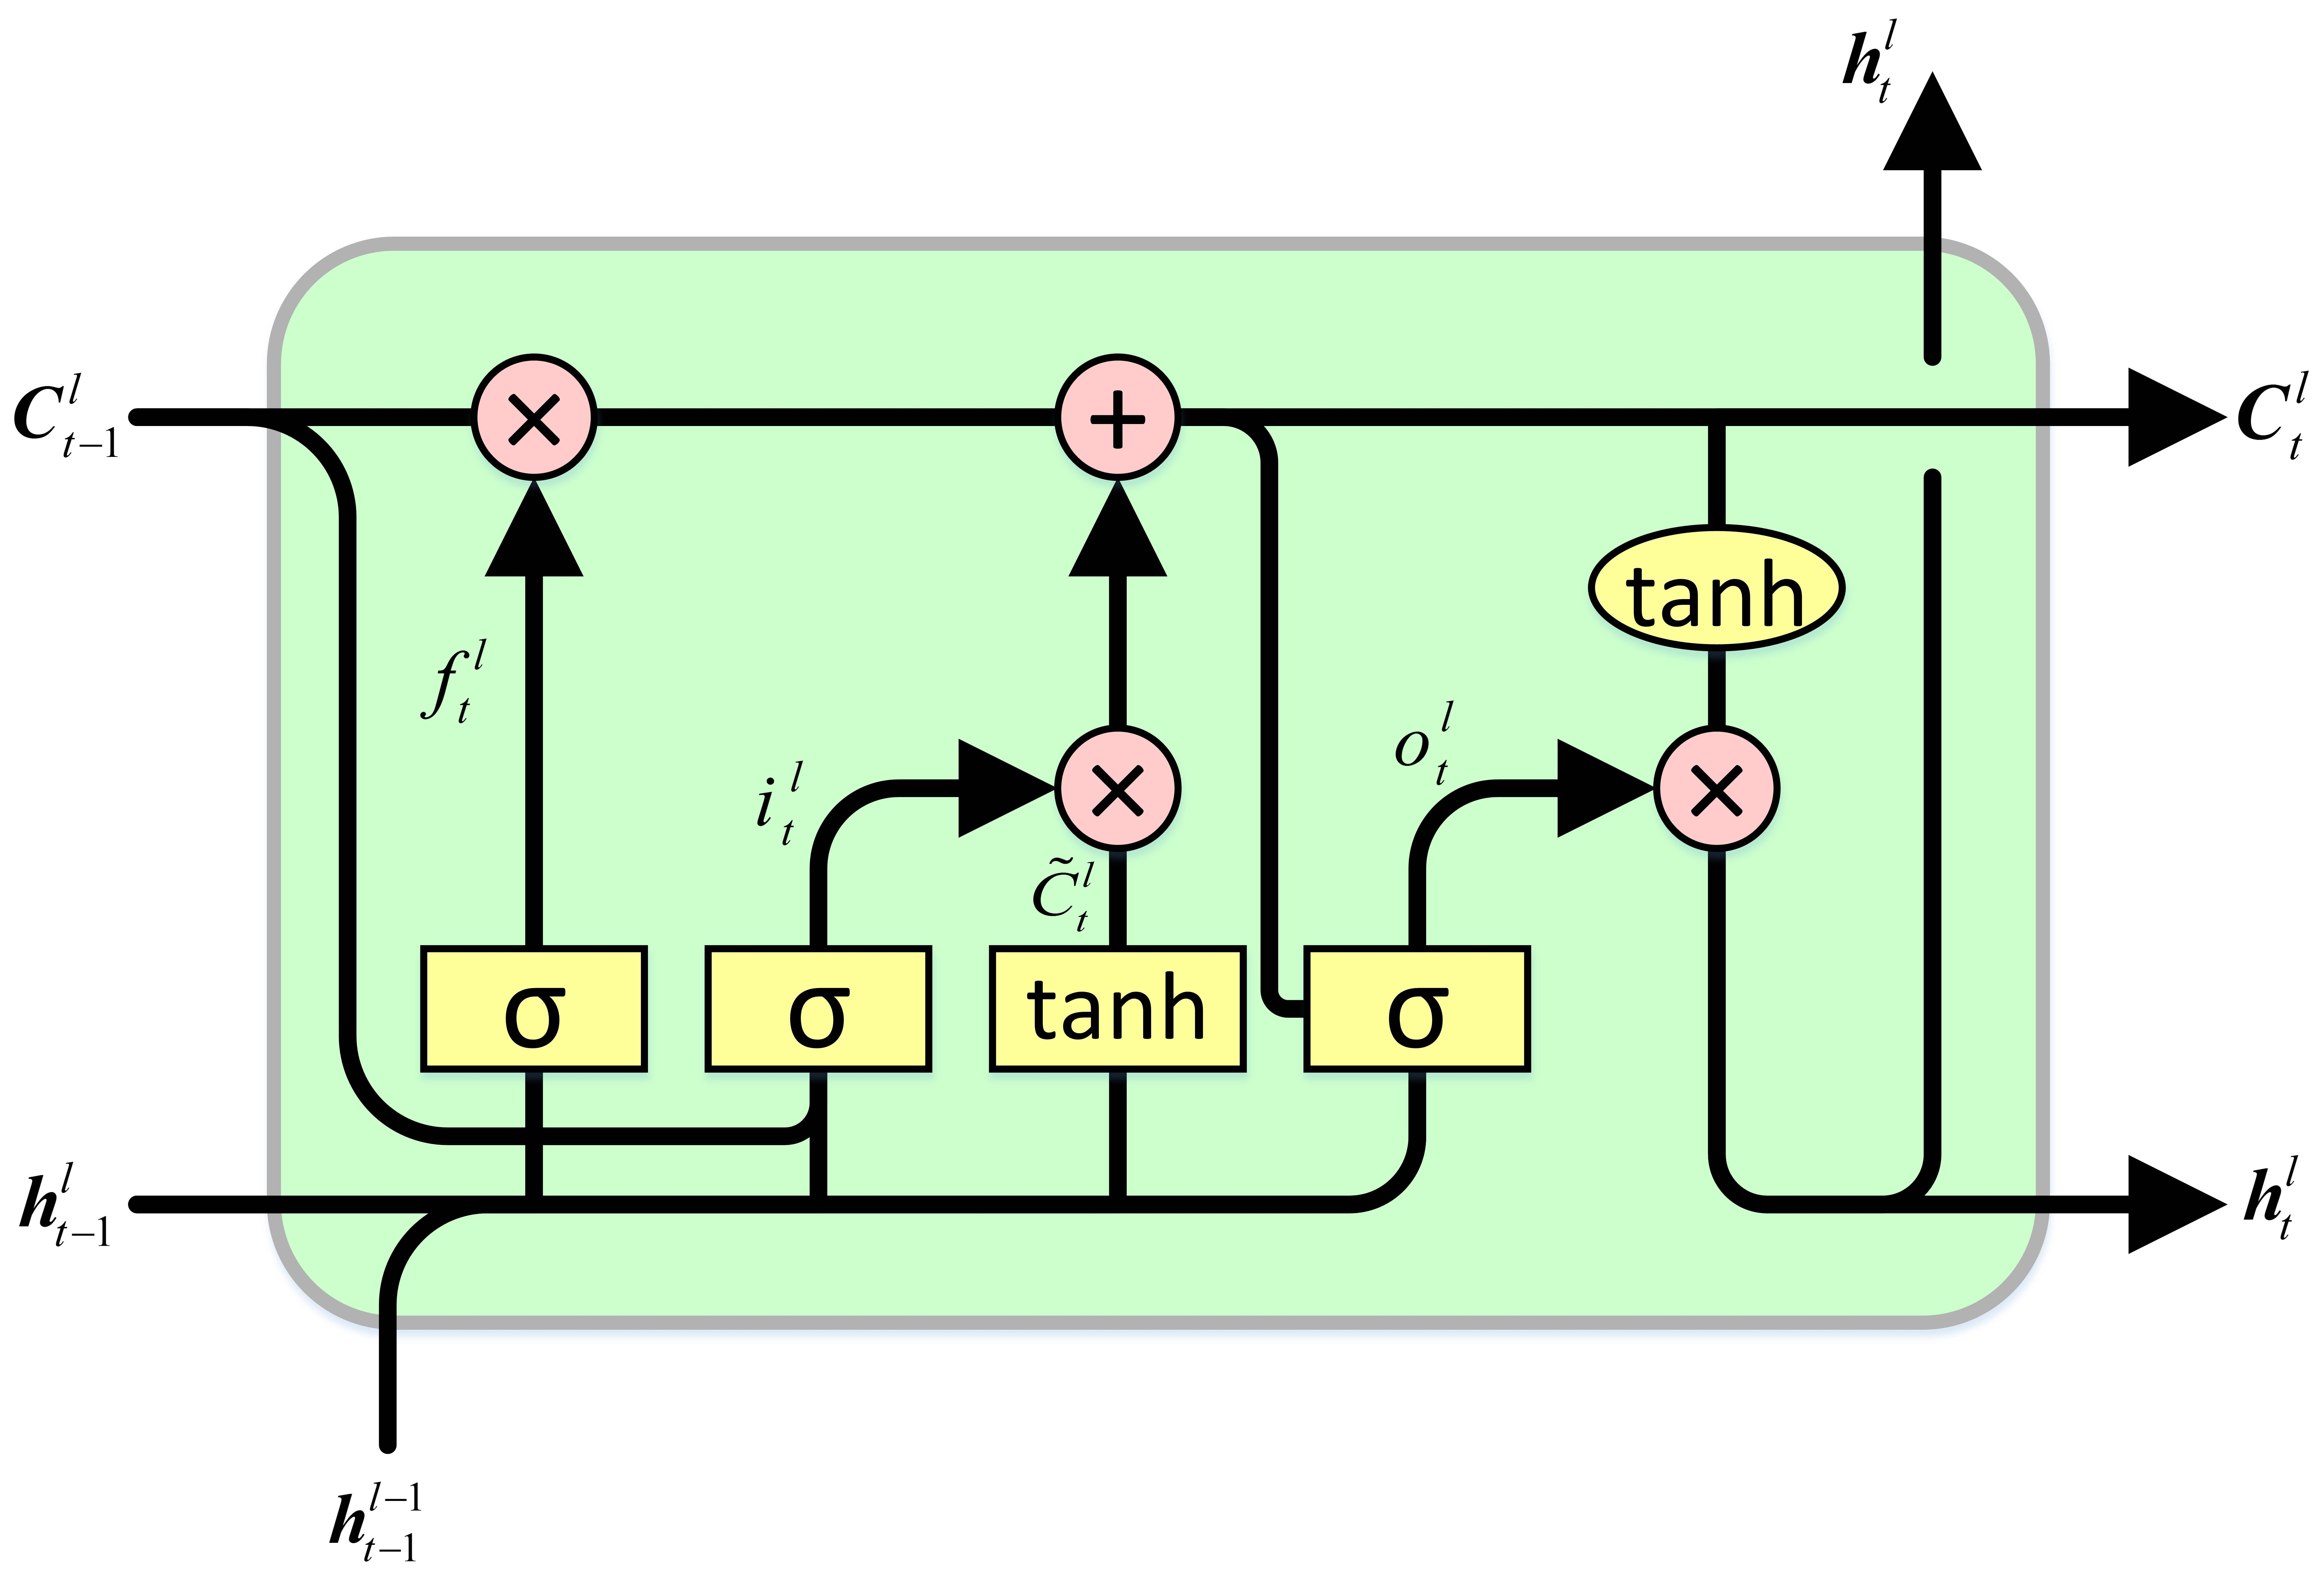
\includegraphics[width=0.75\linewidth]{images/LSTM.png}
    \caption{LSTM Architecture}
    \label{fig:4.5}
\end{figure}


\subsection*{Pseudo code}
\noindent
A pseudo code is a detailed yet readable description of what a computer program or algorithm must do, expressed in a formally-styled natural language rather than in a programming language. It is a high-level description of the actions of a program or algorithm, using a mixture of English and informal programming language syntax. Here is the pseudo code for LSTM algorithm.
\subsection*{Initialization}

\begin{algorithmic}
  \State Initialize weights and biases:
  \State $W_ih \gets initialize\_weights(input\_size, hidden\_size)$
  \State $W_hh \gets initialize\_weights(hidden\_size, hidden\_size)$
  \State $b_ih \gets initialize\_biases(hidden\_size)$
  \State $b_hh \gets initialize\_biases(hidden\_size)$
  \State $W_ho \gets initialize\_weights(hidden\_size, output\_size)$
  \State $b_o \gets initialize\_biases(output\_size)$
\end{algorithmic}

\subsection*{Initial States}
\begin{algorithmic}
  \State Initialize cell\_state and hidden\_state:
  \State $cell\_state \gets initialize\_zeros(hidden\_size)$
  \State $hidden\_state \gets initialize\_zeros(hidden\_size)$
\end{algorithmic}

\subsection*{Forward Pass}
\begin{algorithmic}
  \For{each $input\_t$ in $input\_sequence$}
    \State Calculate input gate, forget gate, cell state, and output gate:
    \State $i_t \gets sigmoid(W_ih \cdot input_t + W_hh \cdot hidden\_state + b_ih + b_hh)$
    \State $f_t \gets sigmoid(W_ih \cdot input_t + W_hh \cdot hidden\_state + b_ih + b_hh)$
    \State $cell\_state \gets f_t \cdot cell\_state + i_t \cdot tanh(W_ih \cdot input_t + W_hh \cdot hidden\_state + b_ih + b_hh)$
    \State $o_t \gets sigmoid(W_ho \cdot hidden\_state + b_o)$
    \State Update hidden\_state:
    \State $hidden\_state \gets o_t \cdot tanh(cell\_state)$
  \EndFor
\end{algorithmic}

\subsection*{Training}
\begin{algorithmic}
  \For{each $epoch$ in $epochs$}
    \For{each $example, label$ in $zip(train\_data, labels)$}
      \State Perform forward pass to get predicted\_output:
      \State $predicted\_output \gets lstm\_forward(example)$
      \State Calculate loss:
      \State $loss \gets compute\_loss(predicted\_output, label)$
      \State Perform backward pass to update weights and biases:
      \State $backward\_pass(loss, learning\_rate)$
    \EndFor
  \EndFor
\end{algorithmic}

\end{document}